% Equivalencia entre convolucion y message passing en grafos
% Compilar con: pdflatex conv_message_passing.tex
\documentclass[tikz,border=10pt]{standalone}
\usepackage{tikz}
\usepackage{amsmath,amssymb}

\usetikzlibrary{arrows.meta, positioning, calc, decorations.pathreplacing}

\definecolor{gdlblue}{RGB}{41, 98, 168}
\definecolor{gdlred}{RGB}{191, 49, 49}
\definecolor{gdlgreen}{RGB}{30, 130, 76}
\definecolor{gdlorange}{RGB}{217, 130, 30}
\definecolor{gdlpurple}{RGB}{118, 56, 138}
\definecolor{gdlgray}{RGB}{140, 140, 140}
\definecolor{gdlyellow}{RGB}{190, 140, 10}

\begin{document}
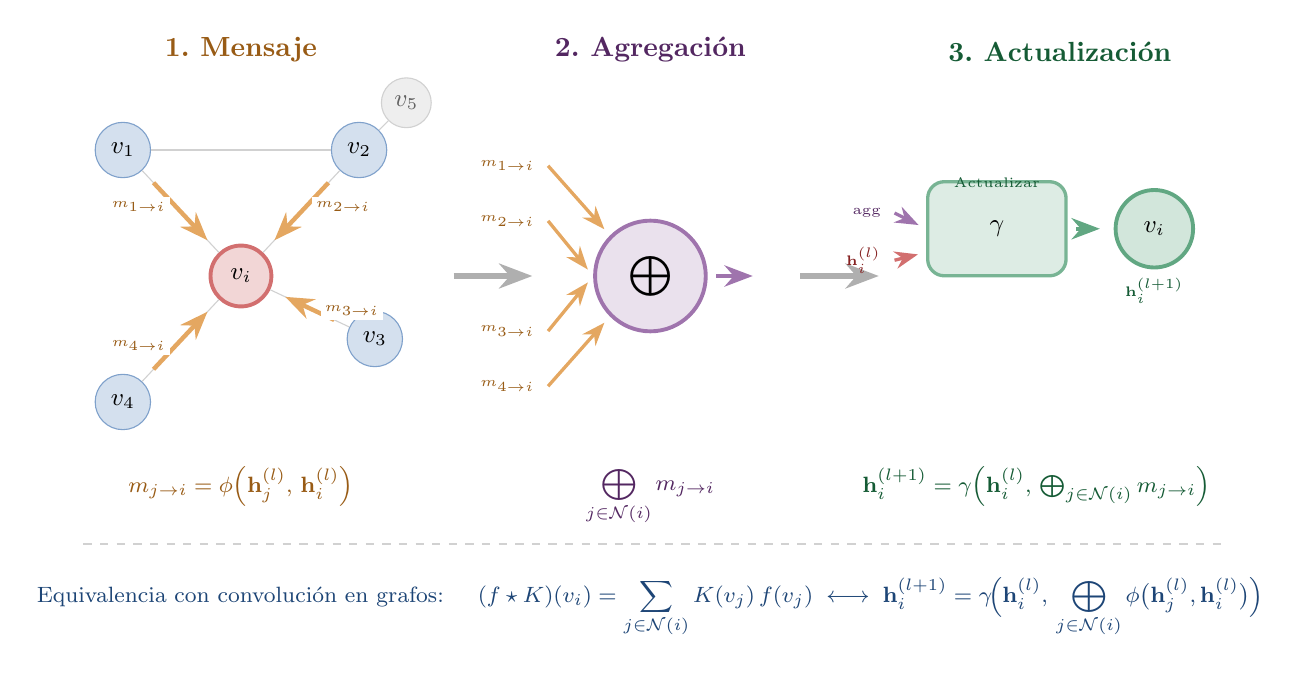
\begin{tikzpicture}[>=Stealth, font=\small]

% ============================================================
% Step labels above each panel
% ============================================================
\node[font=\bfseries, text=gdlorange!70!black, anchor=south] at (1.5, 4.6)
    {1.\ Mensaje};
\node[font=\bfseries, text=gdlpurple!70!black, anchor=south] at (6.7, 4.6)
    {2.\ Agregaci\'{o}n};
\node[font=\bfseries, text=gdlgreen!70!black, anchor=south] at (11.9, 4.6)
    {3.\ Actualizaci\'{o}n};

% ============================================================
% Panel 1: Graph with message passing arrows
% ============================================================
\begin{scope}[shift={(0,0)}]

    % Node styles
    \tikzset{
        centernode/.style={circle, draw=gdlred!70, fill=gdlred!20,
            minimum size=22pt, inner sep=0pt, font=\small\bfseries,
            line width=1.4pt},
        neighnode/.style={circle, draw=gdlblue!60, fill=gdlblue!20,
            minimum size=20pt, inner sep=0pt, font=\small},
        nonneighnode/.style={circle, draw=gdlgray!40, fill=gdlgray!15,
            minimum size=18pt, inner sep=0pt, font=\small,
            text=gdlgray!70!black}
    }

    % Central node v_i
    \node[centernode] (vi) at (1.5, 2.0) {$v_i$};

    % Neighbor nodes
    \node[neighnode] (v1) at (0.0, 3.6) {$v_1$};
    \node[neighnode] (v2) at (3.0, 3.6) {$v_2$};
    \node[neighnode] (v3) at (3.2, 1.2) {$v_3$};
    \node[neighnode] (v4) at (0.0, 0.4) {$v_4$};

    % Non-neighbor node (for context)
    \node[nonneighnode] (v5) at (3.6, 4.2) {$v_5$};

    % Edges among neighbors and non-neighbors (background)
    \draw[gdlgray!40] (v1) -- (v2);
    \draw[gdlgray!40] (v2) -- (v5);
    \draw[gdlgray!40] (v1) -- (vi);
    \draw[gdlgray!40] (v2) -- (vi);
    \draw[gdlgray!40] (v3) -- (vi);
    \draw[gdlgray!40] (v4) -- (vi);

    % Message arrows from neighbors to v_i
    \draw[->, line width=1.6pt, gdlorange!70, shorten >=6pt, shorten <=6pt]
        (v1) -- (vi);
    \node[font=\tiny, text=gdlorange!70!black, fill=white, inner sep=1.5pt,
        anchor=east, xshift=-2pt]
        at ($(v1)!0.45!(vi)$) {$m_{1 \to i}$};

    \draw[->, line width=1.6pt, gdlorange!70, shorten >=6pt, shorten <=6pt]
        (v2) -- (vi);
    \node[font=\tiny, text=gdlorange!70!black, fill=white, inner sep=1.5pt,
        anchor=west, xshift=2pt]
        at ($(v2)!0.45!(vi)$) {$m_{2 \to i}$};

    \draw[->, line width=1.6pt, gdlorange!70, shorten >=6pt, shorten <=6pt]
        (v3) -- (vi);
    \node[font=\tiny, text=gdlorange!70!black, fill=white, inner sep=1.5pt,
        anchor=west, xshift=2pt]
        at ($(v3)!0.45!(vi)$) {$m_{3 \to i}$};

    \draw[->, line width=1.6pt, gdlorange!70, shorten >=6pt, shorten <=6pt]
        (v4) -- (vi);
    \node[font=\tiny, text=gdlorange!70!black, fill=white, inner sep=1.5pt,
        anchor=east, xshift=-2pt]
        at ($(v4)!0.45!(vi)$) {$m_{4 \to i}$};

    % Message function label
    \node[font=\footnotesize, text=gdlorange!70!black, anchor=north, align=center]
        at (1.5, -0.3)
        {$m_{j \to i} = \phi\!\left(\mathbf{h}_j^{(l)},\, \mathbf{h}_i^{(l)}\right)$};

\end{scope}

% ============================================================
% Arrow 1: Left -> Center
% ============================================================
\draw[->, line width=2pt, gdlgray!70]
    (4.2, 2.0) -- (5.2, 2.0);

% ============================================================
% Panel 2: Aggregation
% ============================================================
\begin{scope}[shift={(5.4, 0)}]

    % Aggregation circle with oplus
    \node[circle, draw=gdlpurple!70, fill=gdlpurple!15,
        minimum size=40pt, inner sep=0pt, line width=1.4pt,
        font=\Large] (agg) at (1.3, 2.0) {$\bigoplus$};

    % Incoming labeled arrows from left
    \draw[->, line width=1.2pt, gdlorange!70, shorten >=3pt]
        (0.0, 3.4) -- (agg.north west);
    \node[font=\tiny, text=gdlorange!70!black, anchor=east] at (-0.05, 3.4)
        {$m_{1 \to i}$};

    \draw[->, line width=1.2pt, gdlorange!70, shorten >=3pt]
        (0.0, 2.7) -- (agg.west);
    \node[font=\tiny, text=gdlorange!70!black, anchor=east] at (-0.05, 2.7)
        {$m_{2 \to i}$};

    \draw[->, line width=1.2pt, gdlorange!70, shorten >=3pt]
        (0.0, 1.3) -- (agg.west);
    \node[font=\tiny, text=gdlorange!70!black, anchor=east] at (-0.05, 1.3)
        {$m_{3 \to i}$};

    \draw[->, line width=1.2pt, gdlorange!70, shorten >=3pt]
        (0.0, 0.6) -- (agg.south west);
    \node[font=\tiny, text=gdlorange!70!black, anchor=east] at (-0.05, 0.6)
        {$m_{4 \to i}$};

    % Output arrow
    \draw[->, line width=1.6pt, gdlpurple!70, shorten <=3pt]
        (agg.east) -- (2.6, 2.0);

    % Aggregation formula below
    \node[font=\footnotesize, text=gdlpurple!70!black, anchor=north, align=center]
        at (1.3, -0.3)
        {$\displaystyle\bigoplus_{j \in \mathcal{N}(i)} m_{j \to i}$};

\end{scope}

% ============================================================
% Arrow 2: Center -> Right
% ============================================================
\draw[->, line width=2pt, gdlgray!70]
    (8.6, 2.0) -- (9.6, 2.0);

% ============================================================
% Panel 3: Update step
% ============================================================
\begin{scope}[shift={(9.8, 0)}]

    % Update function box
    \node[rounded corners=6pt, draw=gdlgreen!60, fill=gdlgreen!15,
        minimum width=50pt, minimum height=34pt, inner sep=5pt,
        line width=1.2pt, font=\small, align=center] (upd) at (1.3, 2.6)
        {$\gamma$};
    \node[font=\tiny, text=gdlgreen!70!black, anchor=south] at (1.3, 3.0)
        {Actualizar};

    % Input: aggregated message
    \draw[->, line width=1.2pt, gdlpurple!70, shorten >=3pt]
        (0.0, 2.8) -- (upd.west);
    \node[font=\tiny, text=gdlpurple!70!black, anchor=east] at (-0.05, 2.8)
        {agg};

    % Input: self-features
    \draw[->, line width=1.2pt, gdlred!70, shorten >=3pt]
        (0.0, 2.2) -- ($(upd.west)+(0,-0.3)$);
    \node[font=\tiny, text=gdlred!70!black, anchor=east] at (-0.05, 2.2)
        {$\mathbf{h}_i^{(l)}$};

    % Output: updated node
    \node[circle, draw=gdlgreen!70, fill=gdlgreen!20,
        minimum size=28pt, inner sep=0pt, font=\small\bfseries,
        line width=1.4pt] (vout) at (3.3, 2.6) {$v_i$};
    \node[font=\tiny, text=gdlgreen!70!black, anchor=north] at (3.3, 2.1)
        {$\mathbf{h}_i^{(l+1)}$};

    \draw[->, line width=1.6pt, gdlgreen!70, shorten <=3pt, shorten >=5pt]
        (upd.east) -- (vout);

    % Update formula below
    \node[font=\footnotesize, text=gdlgreen!70!black, anchor=north, align=center]
        at (1.8, -0.3)
        {$\mathbf{h}_i^{(l+1)} = \gamma\!\left(\mathbf{h}_i^{(l)},\,
        \bigoplus_{j \in \mathcal{N}(i)} m_{j \to i}\right)$};

\end{scope}

% ============================================================
% Bottom: Equivalence with convolution
% ============================================================
\draw[gdlgray!40, dashed, line width=0.8pt] (-0.5, -1.4) -- (14.0, -1.4);

\node[font=\footnotesize, text=gdlblue!70!black, anchor=north, align=center]
    at (6.7, -1.7)
    {Equivalencia con convoluci\'{o}n en grafos:
    \quad $\displaystyle (f \star K)(v_i)
    = \sum_{j \in \mathcal{N}(i)} K(v_j)\, f(v_j)
    \;\longleftrightarrow\;
    \mathbf{h}_i^{(l+1)} = \gamma\!\Bigl(\mathbf{h}_i^{(l)},\,
    \bigoplus_{j \in \mathcal{N}(i)}
    \phi\bigl(\mathbf{h}_j^{(l)}, \mathbf{h}_i^{(l)}\bigr)\Bigr)$};

\end{tikzpicture}
\end{document}
